\section{Brief code description}

Σε αυτην την εργασία επιλέχτηκε να γραφεί ο κώδικα για το CNN μοντέλο με την βοήθεια της βιβλιοθήκης numpy.  Συγκεκριμένα γράφηκε κώδικας για τα Dense Layers, Convolutonal Layers, Relu και Softmax Activation, Dropout Layers, Loss function(LossCategoricalCrossEntropy), και τέλος για τους ADAM και SGD optimizers. Οι κώδικες βρίσκονται στο παράρτημα \ref{appendix:app} . Η αρχική ιδέα ήταν να γραφτεί ενα απλό νευρωνικό δίκτυο να δοκιμαστεί σε ένα μικρό dataset και μετά να εμπλουτιστεί αυτο το νευρωνικό με ένα συνελικτικό layer. Υπήρξε μία δυσκολία να δουλέψουν όλα μαζί λόγω προβλημάτων στην μορφη των πινάκων τελικά μπόρεσε και εγίνε το train πάνω στο dataset της MNIST-DIGIT.

\section{Training the model with different optimizers}

Κατά το training επιλέχθηκε να μπεί ενα όριο στα δεδομένα που θα χρησιμοποιηθούν απο την MNIST-DIGIT λόγω χρόνου και μη βελτιστοποιημενου κώδικα να τρέχει σε παραπάνω απο 1 πυρήνες. Συγκεκριμένα επιλέχθηκε να τρέξουν όλα τα διαφορετικά μοντέλα σε $20000$ δεδομένα. Τα μοντέλα είχαν κοινή αρχιτεκτονική (πέρα απο την 3η περίπτωση) αλλά διαφορετικούς optimizer. Στην 1η περίπτωση επιλέχθηκε να γίνεται βελτιστοποίηση μόνο με learning rate = 10e-5. Στην 2η περίπτωση επιλέχθηκε να χρησιμοποιηθεί ο SGD optimizer, με διαφορετικές παραμέτρους. Την 1η φορά έτρεξε το μοντέλο με SGD(learning rate=10e-4, decay=10e-5, momentum=0.5), και την 2η φορά με SGD(learning rate=10e-5, decay=10e-6, momentum=0.9).
Ουσιαστικά μειώθηκαν την 2η φορά το learing rate και το decay ενώ το momentum ανέβηκε.Στην 3ή και τελευταί περίπτωση σύγκρισης των optimizers 
χρησιμοποιήθηκε ο ADAM με learning rate = 10e-5 και decay = 10e-6. Σε όλες τις περιπτώσεις το train πραγματοποιήθηκε για 100 εποχές, ενώ η αρχιτεκτονική του δικτύου ήταν : Convolution Layer((1, 28, 28), 3, 10) - Activation ReLU() - Dropout Layer(0.4) - Reshape((10, 26, 26), (10 * 26 * 26, 1)) - Layer Dense(10 * 26* 26,128) - Activation ReLU() - Dropout Layer(0.5) - Layer Dense(128,10) - Activation ReLU() - Dropout Layer(0.2) - Activation Softmax() - Loss CategoricalCrossentropy(). Στην 3η περίπτωση η αρχιτεκτόνικη άλλαξε, βγάζοντας το Dropout Layer μετά το Convolution Layer, και μειώνοντας το rate του επόμενου σε 0.2


\subsection{Results of the models with different optimizers}

Σέ όλες τις περιπτώσεις μετρήθηκε το training loss/accuracy και το validation loss/accuracy.  

Στο διάγραμμα \ref{f:g1} παρατηρούνται τα αποτελέσματα της 1ής περίπτωσης. Φαίνεται οτι μόνο με learning rate το μοντέλο μαθαίνει αρκετά γρήγορα στις πρωτες 20 εποχές, ενω για τις υπόλοιπες 80 βλέπουμε να μην μπορεί να ξεπεράσει το 80$\%$. Αντίστοιχα το loss του μοντέλου πέφτει απο το 2.0 στο 0.8 τις πρώτες 20 εποχές, και μετά σχεδόν σταθεροποιείται με την τιμη του loss να παραμενει μεταξυ 0.8 και 0.6.

\begin{figure}[ht]
	\centering
	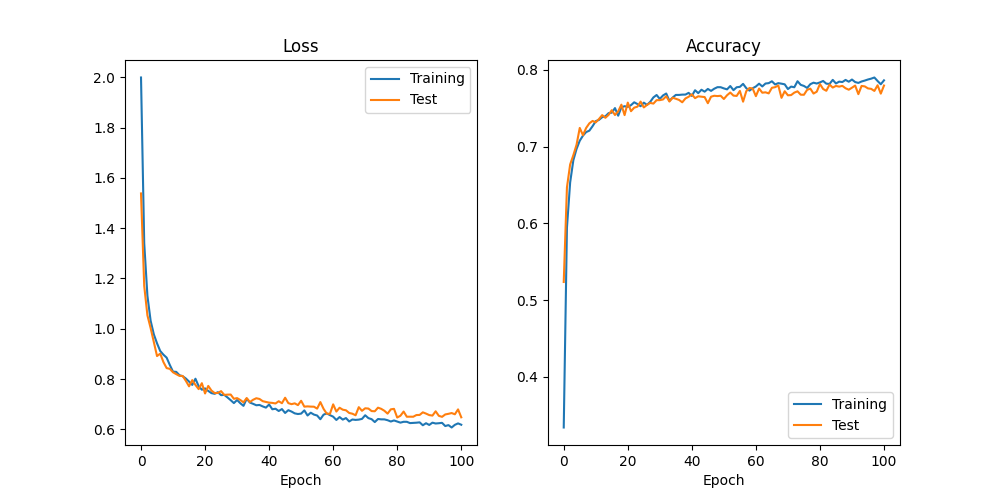
\includegraphics[width=1\linewidth]{Results/Optimizers/lr_20k.png}
	\caption{ Διάγραμμα loss, accuracy για την 1ή περίπτωση εκπαίδευσης του μοντέλου    }
	\label{f:g1}	
\end{figure}


\begin{figure}[ht]
	\centering
	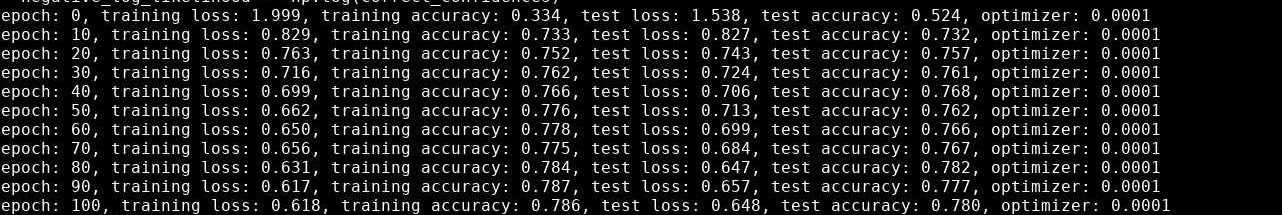
\includegraphics[width=1\linewidth]{Results/Optimizers/lr_20k1.png}
	\caption{Πίνακας εποχών}
	\label{f:g2}	
\end{figure}
\clearpage

Στο διάγραμμα \ref{f:g3} παρατηρούνται τα αποτελέσματα της 2ης περίπτωσης θέτοντας των SGD με τις εξής παραμέτρους : learning rate=10e-4, decay=10e-5, momentum=0.5, ενώ στο δίαγραμμα \ref{f:g5} παρατηρούνται τα αποτελέσματα με SGD(learning rate=10e-5, decay=10e-6, momentum=0.9). Τόσο την 1η φορά οσο και την 2ή παρατηρείται το ίδιο μοτίβό με την προηγούμενη περίπτωση. Τις πρώτες 20 εποχές το loss πέφτει παρα πολύ φτάνοντας σχεδον στο 0.6, ενώ το accuracy αυξανεται παρα πολύ φτάνοντας σχεδόν στο 80$\%$ και μετά παραμένει σχεδον σταθερό. Αυτο φαινεται και στους πίνακες εποχών και των δύο training \ref{f:g4}, \ref{f:g6}.

\begin{figure}[ht]
	\centering
	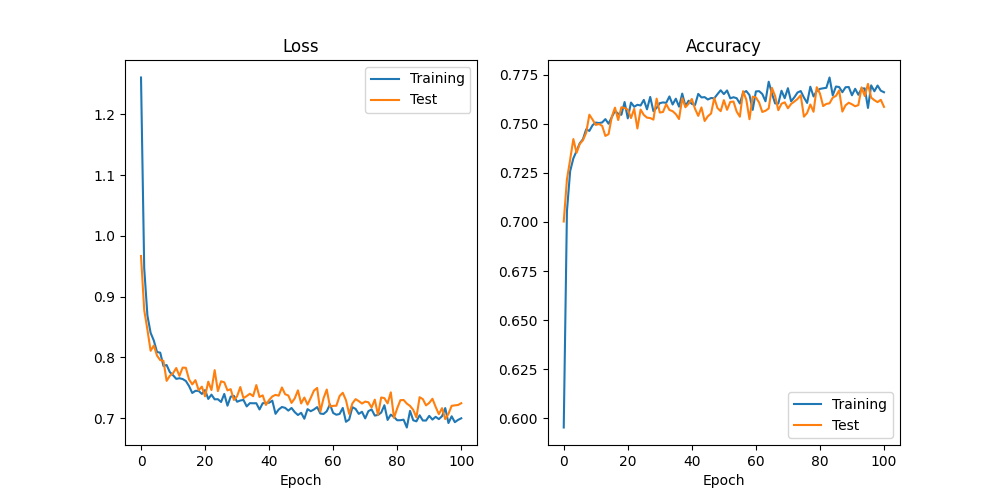
\includegraphics[width=1\linewidth]{Results/Optimizers/optimizer_sgd_20k.png}
	\caption{ Διάγραμμα loss, accuracy για την 2ή περίπτωση εκπαίδευσης του μοντέλου με παραμέτρους : learning rate=10e-4, decay=10e-5, momentum=0.5 }
	\label{f:g3}	
\end{figure}


\begin{figure}[ht]
	\centering
	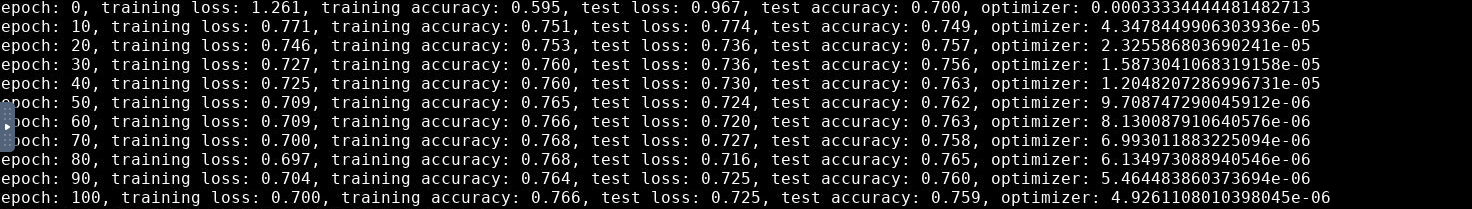
\includegraphics[width=1\linewidth]{Results/Optimizers/optimizer_sgd_20k1.png}
	\caption{Πίνακας εποχών}
	\label{f:g4}	
\end{figure}

\begin{figure}[ht]
	\centering
	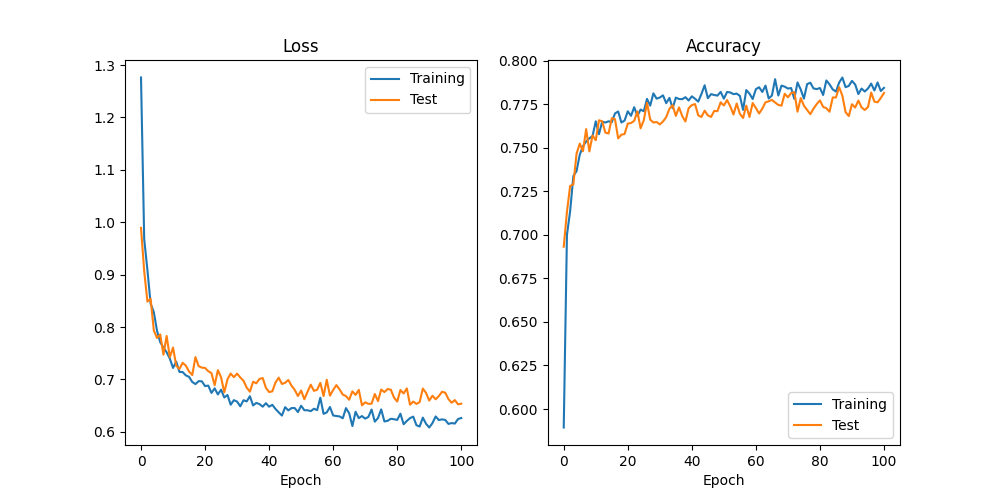
\includegraphics[width=1\linewidth]{Results/Optimizers/optimizer_sgd_2_20k.png}
	\caption{ Διάγραμμα loss, accuracy για την 2ή περίπτωση εκπαίδευσης του μοντέλου με παραμέτρους : learning rate=10e-5, decay=10e-6, momentum=0.8}
	\label{f:g5}	
\end{figure}


\begin{figure}[ht]
	\centering
	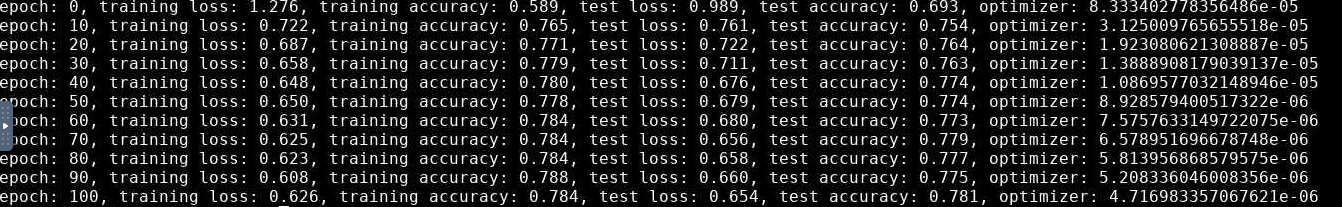
\includegraphics[width=1\linewidth]{Results/Optimizers/optimizer_sgd_2_20k1.png}
	\caption{ Πίνακας εποχών}
	\label{f:g6}	
\end{figure}
\clearpage

Τέλος στο διάγραμμα \ref{f:g7} παρατηρούνται τα αποτελέσματα της 3ης περίπτωσης, δηλαδή την χρήσης ADAM. Στην συγκεκριμένη περίπτωση παρατηρήθηκε κάτι πολυ περίεργο. Όσες φορες και να ετρεξε το μοντέλο, με τον adam για optimizer, πάντα κολλούσε το training είτε στην αρχη με 10$\%$ είτε όπως βλέπουμε και στο διάγραμμα \ref{f:g7} , όπου ξεκινάει με ένα καλό accuracy ανεβαίνει γρηγορα μετα σταθεροποιείται για λίγο ξανα αναβαινει και παραμένει σχεδόν σταθερό.Η διαφορά με τα άλλα δυο μοντέλα είναι ότι 
αυτό εξαρτάται πάρα πολύ απο την αρχικοποίηση των βαρών των Layers, κατι που μπορεί να το κολλήσει και να βγάλει ένα διάγραμμα σαν αυτό \ref{f:g8}. Παρόλο που στο συγκεκριμένο διάγραμμα το μοντέλο εκπαιδέυτηκε σε 10000 δεδομένα, παρόμοια αποτελέσματα παρατηρήθηκαν και με παραπάνω δεδομένα. Ποσοστό επιτυχίας άνω του 50 $\%$ δεν παρατηρήθηκε ποτέ ακόμα και με την αρχιτεκτονική των προηγούμεων περιπτώσεων.


\begin{figure}[ht]
	\centering
	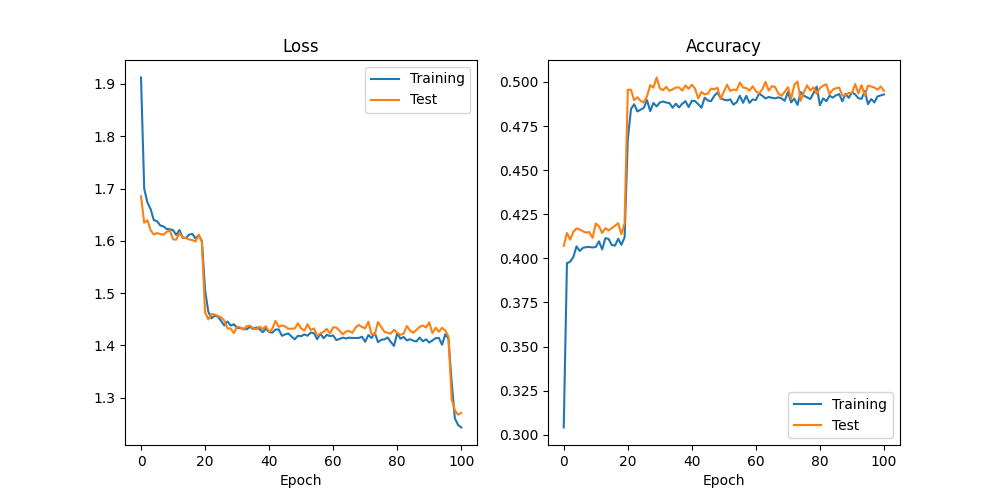
\includegraphics[width=1\linewidth]{Results/Optimizers/without_dropout_adam_20k.png}
	\caption{ Διάγραμμα loss, accuracy για την 3ή περίπτωση εκπαίδευσης του μοντέλου για 20k δεδομενα}
	\label{f:g7}	
\end{figure}


\begin{figure}[ht]
	\centering
	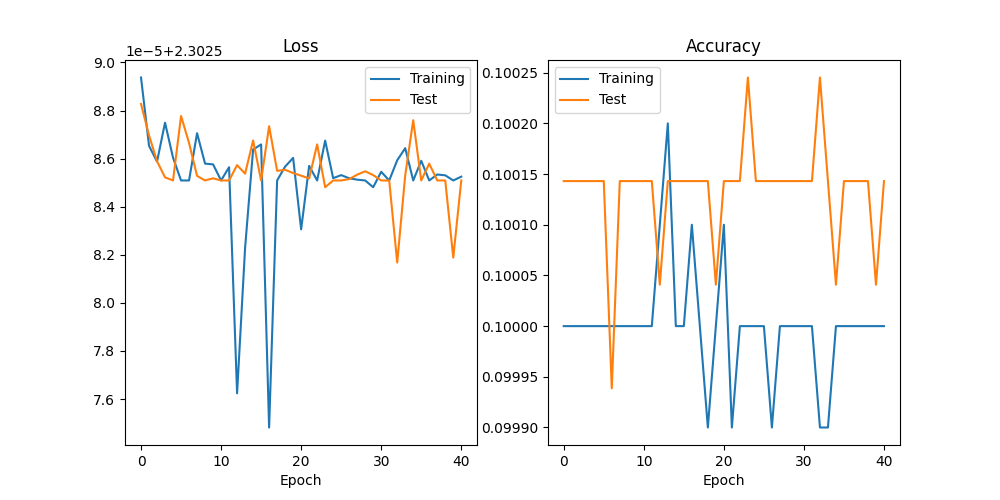
\includegraphics[width=1\linewidth]{Results/Optimizers/without_dropout_adam_10k.png}
	\caption{ Διάγραμμα loss, accuracy για την 3ή περίπτωση εκπαίδευσης του μοντέλου για 10k δεδομένα}
	\label{f:g8}	
\end{figure}
\clearpage

\section{Conclusion}

Στην συνεχεια, επιλέχθηκε ο στοχαστικός (SGD) με παραμέτρους learning rate=10e-5, decay=10e-6, momentum=0.8, με την αρχιτεκτονική του δικτύου που χρησιμοποιήθηκε στον ADAM με την μόνη αλλαγη να βρισκεται στο Convolution Layer, όπου οι kernels αυξηθηκαν απο 10 σε 64 : Convolution Layer((1, 28, 28), 3, 64). Αυτό το μοντέλο επιλέχθηκε να εκπαιδευτει σε 40000 δεδομένα στην MNIST-DIGIT και να συγκριθεί με το αντιστοιχο δίκτυο γραμμένο στην tensorflow. 

